% !TEX root = ../Thesis.tex

\chapter{Gestione della memoria}
Questo capitolo esplorerà nel dettaglio come Java e Rust affrontano il tema della gestione della memoria. I due linguaggi adottano due filosofie molto diverse:
\begin{itemize}
    \item Java affida al \textit{Garbage Collector(GC)} il compito di liberare la memoria automaticamente, semplificando lo sviluppo ma introducendo overhead. 
    \item Rust elimina il GC grazie a un sistema di \textit{ownership} e \textit{borrowing}, garantendo deallocazione deterministica e sicurezza a compile-time. 
\end{itemize}
\section{L'approccio di Java}
Java è un linguaggio di programmazione progettato per essere semplice, portabile e sicuro, con una gestione della memoria che mira ridurre la complessità e prevenire errori comuni legati all'uso diretto delle risorse. Java raggiunge questi obiettivi affidando l'intera gestione della memoria alla Java Virtual Machine (JVM). Gli aspetti fondamentali dell'approccio di Java sono:

\begin{enumerate}
\item L'allocazione automatica della memoria tramite JVM: gli oggetti vengono creati dinamicamente nell'heap senza che il programmatore debba preoccuparsi di allocare la memoria manualmente. 
\item La gestione deallocazione automatica tramite il garbage collector, una componente della JVM che si occupa di individuare e liberare la memoria occupata da oggetti non più raggiungibili, prevenendo così problemi comuni, come i memory leak o dangling pointer. Questo, di fatto, toglie al programmatore la responsabilità collegata al dover gestire manualmente la deallocazione della memoria, riducendo la probabilità di errori nel codice.
\item La prevenzione di comportamenti indefiniti a run-time, attraverso un controllo rigoroso dell'accesso alla memoria a runtime: ad esempio, accessi a riferimenti nulli generano eccezioni gestibili da parte dello sviluppatore. 
\end{enumerate}

Tuttavia, l'approccio automatico della gestione della memoria porta alcuni svantaggi per quanto riguarda le prestazioni del programma. Il garbage collector, infatti, introduce un overhead significativo, poiché deve periodicamente eseguire la scansione della memoria per identificare gli oggetti non più raggiungibili e liberare la memoria occupata da essi. Questo processo può causare pause impreviste nell'esecuzione del programma, che possono essere problematiche quando si richiedono alte prestazioni. La JVM moderna implementa algoritmi di garbage collection avanzati per cercare di ridurre al minimo le interruzioni e ottimizzare le prestazioni, ma il costo di queste operazioni rimane comunque un fattore da considerare. 
\section{L'approccio di Rust}
Rust è un linguaggio di programmazione moderno progettato per garantire sicurezza nella gestione della memoria senza fare uso di un garbage collector. Rust ha due obiettivi principali:
\begin{enumerate}
    \item  Garantire che il programma sia privo di comportamenti indefiniti, ovvero situazioni in cui il programma può agire in modo imprevedibile. Un esempio tipico è l'accesso a memoria non valida, che può portare all'esecuzione di codice con dati non inizializzati o causare errori di memoria come segmentation fault. 
    \item Eseguire la prevenzione di comportamenti indefiniti a compile-time, piuttosto che a run-time. Questo significa che il compilatore di Rust è in grado di rilevare e segnalare errori di memoria prima che il programma venga eseguito, riducendo il rischio di bug e di errori durante l'esecuzione. 
    % Nell'articolo di google viene riportato il vantaggio di non avere controlli a run-time.
\end{enumerate}
Rust raggiunge questi obiettivi attraverso un sistema di gestione della memoria basato su \textit{ownership} e \textit{borrowing}, concetti affrontati nelle prossime sezioni. L'approccio di Rust consente di evitare interamente classi di errori comuni nei linguaggi tradizionali: buffer overflow, dangling pointer, race condition sui dati condivisi. Inoltre, poiché questi controlli vengono effettuati a compile-time, Rust riduce drasticamente la necessità di controlli a run-time, migliorando le prestazioni senza sacrificare la sicurezza. 

Rust non può prevenire tutti i possibili bug ma le metodologie messe in atto per la gestione della memoria rendono un programma scritto in Rust molto più sicuro rispetto a uno scritto in linguaggi con meno controlli. Un esempio concreto è fornito da Google \cite{android13-memorysafe}, che ha introdotto il linguaggio nello sviluppo di Android 13. In particolare, circa il 21\% del nuovo codice introdotto in Android 13 è stato scritto in Rust, e, alla data della pubblicazione dell'articolo, non sono state scoperte vulnerabilità di sicurezza legate alla memoria in questo codice. Questo è un risultato significativo che dimostra come gli obiettivi prefissati da Rust siano stati raggiunti nella pratica.

Rust realizza questi obiettivi attraverso un sistema basato sui concetti di \textit{ownership} e \textit{borrowing}. Concetti fondamentali che verrano affrontati in dettaglio nelle prossime sezioni.

\section{Stack e Heap}
Sia Java che Rust utilizzano due aree di memoria principali: lo stack e l'heap, ma la loro gestione è profondamente diversa, riflettendo i diversi modelli di memoria adottati dai due linguaggi.

Lo stack è un'area di memoria strutturata con una struttura dati stack LIFO (Last In, First Out). La memoria stack è contigua e i dati memorizzati al suo interno sono in posizione fissa rispetto allo stack pointer, un puntatore che punta all'ultimo elemento inserito. Questo permette un accesso rapido ai dati usando indirizzi di memoria calcolati in modo semplice tramite un offset rispetto allo stack pointer. Inoltre, allocazione e deallocazione della memoria stack sono molto veloci poiché avvengono spostando lo stack pointer, avanti o indietro, di un numero di byte opportuno rispetto alla dimensione del dato e all'architettura della CPU.

L'heap, al contrario, è un'area di memoria in cui i dati possono essere allocati in qualsiasi sua posizione. L'allocazione e la deallocazione della memoria heap richiedono operazioni più complesse rispetto allo stack, poiché il sistema operativo deve tenere traccia degli spazi liberi e occupati. Questo può portare a un utilizzo meno efficiente della memoria (frammentazione) e a un accesso più lento ai dati rispetto allo stack. 

In Java, l'allocazione della memoria è fortemente automatizzata. Ogni volta viene creato un oggetto, tramite la keyword \texttt{new}, viene allocata dinamicamente memoria heap nel quale sarà memorizzato l'oggetto. L'uso dello stack è limitato a variabili di tipo primitivo e variabili locali. Al contrario, Rust adotta un modello più esplicito e flessibile. In rust, la variabili possono essere allocate sia nello stack che nell'heap, a seconda dalla conoscenza a compile time delle dimensioni del dato:
\begin{itemize}
    \item  Se la variabile ha una dimensione fissa nota a compile time, viene allocata nello stack. É possibile allocare nell'heap anche variabili di dimensione fissa attraverso \texttt{Box}\footnote{\texttt{Box<T>} è uno smart pointer fornito dalla standard library di Rust che consente di allocare un valore di tipo \texttt{T} sull'heap.}.
    \item  Se la variabile ha una dimensione variabile o non nota a compile time, viene allocata nell'heap. 
\end{itemize} 
Questa è una differenza fondamentale rispetto a Java, perchè permette allo sviluppatore di avere più controllo su dove vengono allocati i dati, permettendo ottimizzazioni specifiche per le esigenze del programma. 

Ad esempio, sia in Java che in Rust, gli array hanno una dimensione fissa. Tuttavia, in Java, gli array sono allocati nell'heap e sono referenziati da variabili nello stack, mentre in Rust, poiché si conosce la loro dimensione a compile time, vengono allocati nello stack. Questo rende l'accesso agli elementi dell'array di Rust più veloce. 
\begin{minted} [fontsize=\small] {Java}
    int[] arr = {1, 2, 3, 4, 5}; // Array allocato nell'heap
    System.out.println("Il primo elemento e': " + arr[0]);
\end{minted}
\begin{minted} [fontsize=\small] {Rust}
    let arr = [1, 2, 3, 4, 5]; // Array allocato nello stack
    println!("Il primo elemento e': {}", arr[0]);
\end{minted}
\section{Ownership}
L'ownership è un concetto fondamentale di Rust il quale può essere definito come un insieme di regole che il compilatore controlla per garantire una corretta gestione della memoria. Questo significa sia garantire che non ci siano errori di memoria a run-time, sia che la memoria inutilizzata venga rilasciata correttamente per non terminare lo spazio di memoria disponibile. 

L'obiettivo principale dell'ownership è, quindi, quello di gestire la memoria heap tenendo traccia di quali parti di codice utilizzano valori contenuti in essa, minimizzare valori duplicati e garantire che la memoria venga rilasciata quando non è più necessaria. 
%TODO: Forse inserire confronto con Java su performance e garbage collector 

L'ownership si basa su tre regole principali: 
\begin{enumerate}
    \item  Ogni valore in Rust ha un \textit{owner}, ovvero una variabile che ne detiene la proprietà. 
    \item  Un valore può avere un solo owner alla volta. 
    \item  Quando l'owner di un valore esce dallo scope, il valore viene automaticamente rilasciato dalla memoria.
\end{enumerate}
Consideriamo un caso banale in cui si crea una variabile all'interno di uno scope:
\begin{minted} [fontsize=\small] {Rust}
    {
        let s = String::from("Hello");
    }
\end{minted}
In questo caso, secondo la regola 3, quando la variabile \texttt{s} esce dallo scope, il valore \texttt{"Hello"} viene automaticamente rilasciato dalla memoria. Questo avviene attraverso la funzione \texttt{drop} che viene chiamata automaticamente da rust quando la variabile esce dallo scope. In Java questo non accade. Dato il seguente codice equivalente in Java:
\begin{minted} [fontsize=\small] {Java}
    {
        String s = new String("Hello");
    }
\end{minted}
La memoria occupata dalla stringa \texttt{"Hello"} non viene rilasciata automaticamente quando \texttt{s} esce dallo scope, ma solo quando il garbage collector esegue la raccolta dei valori non più raggiungibili. Già da questo semplice caso si può notare come l'ownership di Rust permetta di avere un controllo più preciso sulla memoria. 

Un altro aspetto importante dell'ownership è che, quando si assegna un valore a un'altra variabile, l'ownership viene trasferita. Ad esempio, consideriamo il seguente codice:
\begin{minted} [fontsize=\small] {Rust}
    let s1 = String::from("Hello");
    let s2 = s1; // Ownership di s1 viene trasferita a s2
    println!("{}", s1); // Errore di compilazione
    println!("{}", s2);
\end{minted}
In questo caso, l'ownership della stringa \texttt{"Hello"} viene trasferita da \texttt{s1} a \texttt{s2}. Dopo il trasferimento, \texttt{s1} non è più valida e qualsiasi tentativo di accedervi causerà un errore di compilazione. 
\begin{figure}[h]
    \label{fig:own1}
    \centering
    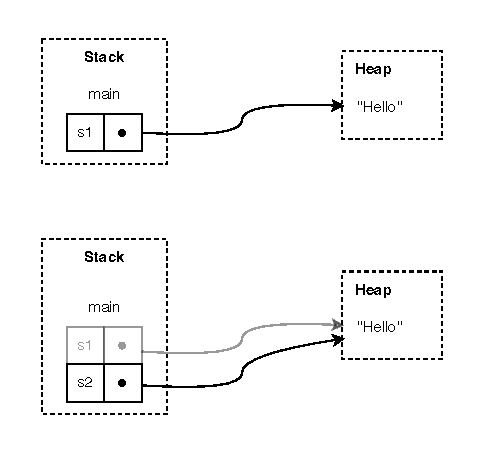
\includegraphics[scale = 1]{Figures/own1.drawio.pdf}
    \caption{Visualizzazione memoria Rust dopo il trasferimento di ownership.}
\end{figure}
In Rust, per variabili il cui valore è contenuto in memoria heap, un'istruzione di copia esegue una \textit{shallow copy} del valore e invalida la variabile originale. Questo comportamento prende il nome di \textit{move}. L'operazione di move è a tutti gli effetti come un trasferimento di proprietà legale, dove il vecchio proprietario non può più accedere alla proprietà venduta. Rust non esegue mai una \textit{deep copy} di una variabile: se il programmatore desidera duplicare effettivamente il contenuto, deve farlo in modo esplicito (ad esempio usando il metodo \texttt{clone()}). Quindi, l'operazione di copia base è poco costosa in termini di performance.

Questo non è consistente con quello che accade in Java, dove l'assegnazione di un oggetto a un'altra variabile non invalida quella originale, ma crea una nuova referenza all'oggetto esistente. Entrambe le variabili possono accedere all'oggetto, condividendone lo stato. In Java, il codice equivalente sarebbe:
\begin{minted} [fontsize=\small] {Java}
    String s1 = "Hello";
    String s2 = s1; 
    System.out.println(s1); // Valido
    System.out.println(s2); // Valido
\end{minted}
In questo caso, quindi, entrambe le stringhe verrebbero correttamente stampate. L'approccio adottato da Rust è decisamente più restrittivo, ma si tratta di una caratteristica desiderabile: consente infatti di evitare errori comuni legati alla gestione della memoria, come l'accesso a variabili non più valide o la modifica involontaria di dati condivisi. 
\subsubsection {Ownership e funzioni}
Il meccanismo di passaggio degli argomenti a funzione in Rust è strettamente legato al concetto di ownership. Quando si passa una variabile a una funzione, l'ownership di quella variabile viene trasferita alla funzione, rendendo, quindi, la variabile originale non più utilizzabile dopo la chiamata. Questo avviene perché Rust utilizza il \textit{pass-by-value}. Ad esempio, consideriamo il seguente codice:
\begin{minted} [fontsize=\small] {Rust}
    fn main() {
        let s1 = String::from("Hello");
        // Ownership di s1 viene trasferita a print_string
        print_string(s1); 
        println!("{}", s1); // Errore di compilazione
    }

    fn print_string(s: String) {
        println!("{}", s);
    }       
\end{minted}
Ciò che accade è: la variabile \texttt{s1} viene passata alla funzione \texttt{print\_string}, ossia \texttt{s1} viene copiata in \texttt{s} e, quindi, l'ownership dei dati di \texttt{s1} passa a \texttt{s}. Come risultato, \texttt{s1} non è più valida dopo la chiamata alla funzione, e qualsiasi tentativo di accedervi causerà un errore di compilazione. 

Java, come Rust, utilizza il \textit{pass-by-value}, ma il passaggio di un oggetto a una funzione non invalida la variabile originale, questo può portare a situazioni sgradevoli.
\begin{listing}[h]
    \begin{minted} [fontsize=\small] {Java}
        class Person {
            private String name;
            public Person(String name) {
                this.name = name;
            }

            public void setName(String name) {
                this.name = name;
            }

            public String getName() {
                return name;
            }
        }

        public class Main {
            public static void main(String[] args) {
                Person p1 = new Person("Alice");
                Person p2 = p1;
                p2.setName("Bob"); // Modifica il nome di p2
                System.out.println(p1.getName()); // Stampa "Bob"
            }
        }
    \end{minted}
    \caption{Modifica di un oggetto tramite un riferimento in Java.}
    \label{lst:java-reference}
\end{listing}
Nell'esempio (\ref{lst:java-reference}), la modifica del campo \texttt{name} di \texttt{p2} influisce anche \texttt{p1}, poiché entrambi i riferimenti puntano allo stesso oggetto in memoria. Questo comportamento può causare bug sottili e difficili da individuare, specialmente in contesti complessi o concorrenti\footnote{È utile notare che, in Java, la keyword \texttt{final} può essere utilizzata per dichiarare una variabile come immutabile. Tuttavia, \texttt{final} non rende immutabile l'oggetto a cui la variabile si riferisce: i campi dell'oggetto possono ancora essere modificati tramite metodi mutator.}. In Rust, invece, il trasferimento di ownership impedisce il comportamento appena descritto, poiché, una volta che l'ownership è stata trasferita, la variabile originale non può più essere utilizzata.

È importante sottolineare che la semantica del \textit{move} in Rust, così come descritta finora, si applica ai tipi di dati che allocano memoria sull'heap, come \texttt{String} o \texttt{Vec}. In questi casi, un'assegnazione o il passaggio a una funzione comporta il trasferimento dell'ownership, e quindi l'invalidazione del valore originale. Tuttavia, per tipi primitivi e a dimensione fissa nota a compile time, come gli interi (\texttt{i32}, \texttt{u64}, etc.), Rust applica una semantica diversa: questi tipi implementano automaticamente il trait \texttt{Copy}. Ciò significa che, in fase di assegnazione o di passaggio come parametro a una funzione, viene eseguita una copia bit a bit del valore, e l'ownership non viene trasferita.

Di conseguenza, entrambi i valori (l'originale e la copia) restano validi e utilizzabili, senza causare errori di compilazione. Ecco un esempio:
\begin{minted}[fontsize=\small]{rust}
    fn main() {
        let x = 42;
        print_value(x); // x viene copiato, non spostato
        println!("{}", x); // x è ancora valido
    }

    fn print_value(n: i32) {
        println!("{}", n);
    }
\end{minted}
Questa distinzione riflette chiaramente la filosofia di Rust nel garantire la sicurezza nell'accesso alla memoria:
\begin{itemize}
    \item Per i tipi che contengono dati allocati dinamicamente o che possono essere modificati a runtime, Rust usa la semantica del \textit{move}, che impedisce di accedere a un valore dopo che la sua \textit{ownership} è stata trasferita altrove, evitando così potenziali problemi di accesso concorrente o modifiche inattese.
    \item Per i tipi con dimensione fissa e nota a compile time, che risiedono interamente nello stack, solitamente immutabili per definizione (come interi o booleani) \footnote{In Rust le variabili sono immutabili a meno che non si vengano dichiarate con la keyword \texttt{mut}.}, Rust utilizza la semantica del \textit{copy}, poiché la copia bit-a-bit è efficiente e non introduce rischi di inconsistenza o accessi errati.
\end{itemize}
L'ownership può essere trasferita anche con le funzioni che ritornano un valore. In questo caso, un assegnamento a una variabile di un valore restituito da una funzione comporta il trasferimento dell'ownership dalla funzione alla variabile. Ad esempio:
\begin{minted}[fontsize=\small]{rust}
    fn main() {
        let s1 = create_string(); 
        println!("{}", s1);
    }

    fn create_string() -> String {
        String s = String::from("Hello from function")
        s // Ownership di s viene trasferita a s1
    }
\end{minted}
L'ownership di una variabile segue sempre lo stesso principio: assegnare il valore a un'altra variabile trasferisce l'ownership. Quando una variabile che include dati nell'heap esce dallo scope, il compilatore chiama automaticamente la funzione \texttt{drop} per rilasciare la memoria occupata da quei dati, a meno che l'ownership non sia stata trasferita a un'altra variabile.
\begin{listing}[H]
    \begin{minted}[fontsize=\small]{rust}
        fn main() {
            let v1 = vec![10, 20, 30];
            let (v2, sum) = sum_vector(v1); 
            println!("La somma degli elementi di {:?} è {}", v2, sum);
        }

        fn sum_vector(v: Vec<i32>) -> (Vec<i32>, i32) {
            let sum = v.iter().sum();
            (v, sum)
        }
    \end{minted}
    \caption{Trasferimento di ownership con ritorno di valore.}
    \label{lst:ownership-return}
\end{listing}

Quindi, se volessimo passare un valore a una funzione e riutilizzarlo dopo la chiamata, dovremmo ritornare quel valore al termine della funzione, eventualmente, in aggiunta ad altri valori che la funzione calcola\footnote{Questo può essere fatto tramite il tipo \texttt{Tuple}: un array di dimensione fissa in cui è possibile memorizzare dati di tipo diverso}(vedi esempio (\ref{lst:ownership-return})). 

\section{Borrowing}
É evidente come l'ownership sia un concetto potente per la gestione della memoria, ma che risulta troppo restrittivo e macchinoso in situazioni come quella riportata nel codice (\ref{lst:ownership-return}). Rust per risolvere questo problema introduce il concetto di \textit{borrowing}, che consente di prendere in prestito un valore senza trasferirne l'ownership, consentendo una maggiore flessibilità. Il borrowing è realizzato attraverso il concetto di riferimento. Il riferimento in Rust non ha le stesse proprietà di un riferimento in Java: 
\begin{itemize}
    \item In Java un riferimento è l'indirizzo di memoria di un oggetto, e può essere utilizzato per accedere e modificare l'oggetto stesso. 
    
    Inoltre, può assumere il valore \texttt{null}, ossia non punta a un oggetto in memoria. Questo ha gravi ripercussioni sulla sicurezza del programma, poiché l'accesso a un riferimento \texttt{null} può causare un \texttt{NullPointerException} a run-time. 
    
    Lo stesso creatore della nozione di riferimento \texttt{null}, Tony Hoare, lo ha definito "billion dollar mistake"\cite{hoare-null-reference}, a causa dei costi che le aziende devono, e dovranno, sostenere per bug e vulnerabilità dovuti a \texttt{null}.
    \item In Rust, un riferimento è anch'esso l'indirizzo di memoria di un valore (mutabile o immutabile). Tuttavia, a differenza di Java, un riferimento in Rust non può essere \texttt{null}. Il compilatore di Rust garantisce che ogni riferimento punti sempre a un valore valido di un tipo specifico per tutta la durata della sua esistenza. Questo dà importanti garanzie di sicurezza, poiché elimina la possibilità di avere errori a run-time legati a riferimenti nulli.
    %TODO: inserire come rust gestisce l'assenza di valore 
\end{itemize}
I riferimenti in Rust sono ottenuti utilizzando l'operatore di referenziazione \texttt{\&} che restituisce il riferimento alla variabile su cui viene applicato. Ad esempio:
\begin{minted}[fontsize=\small]{rust}
    fn main() {
        let s1 = String::from("Hello");
        print_string(&s); 
    }
    fn print_string(s2: &String) {
        println!("{}", s2);
    }
\end{minted} 
In questo esempio, \texttt{s1} è una variabile che si trova nello stack e contiene un valore allocato nell'heap. Pertanto, quando si applica l'operatore \texttt{\&} a \texttt{s1}, si ottiene un riferimento a una variabile sullo stack. Quindi, si hanno due livelli di indirezione: \texttt{s2} per poter accedere a \texttt{"Hello"} deve prima seguire il riferimento a \texttt{s1} e poi accedere al valore allocato nell'heap.  
\begin{figure}[H]
    \label{fig:bor1}
    \centering
    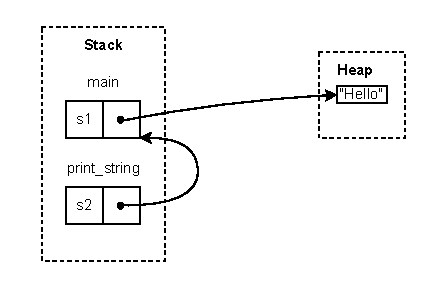
\includegraphics[scale = 1]{Figures/bor1.drawio.pdf}
    \caption{Visualizzazione memoria Rust durante la chiamata di \texttt{print\_string()}.}
\end{figure} 
In Java, non è possibile avere questo livello di indirezione, poiché i riferimenti puntano direttamente a oggetti in memoria. Infatti, il codice equivalente in Java sarebbe:
\begin{minted}[fontsize=\small]{Java}
    public class Main {
        public static void main(String[] args) {
            String s1 = "Hello";
            printString(s1); 
        }
        public static void printString(String s2) {
            System.out.println(s2);
        }
    }
\end{minted}
In questo caso, \texttt{s1} e \texttt{s2} sono entrambi riferimenti all'oggetto \texttt{"Hello"} in memoria.
\begin{figure}[H]
    \label{fig:bor2}
    \centering
    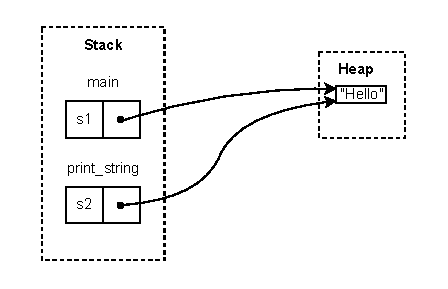
\includegraphics[scale = 1]{Figures/bor2.drawio.pdf}
    \caption{Visualizzazione memoria Java durante la chiamata di \texttt{printString()}.}
\end{figure} 
Per eseguire l'operazione opposta, ossia ottenere il valore a cui punta un riferimento, si utilizza l'operatore di dereferenziazione \texttt{*}. 

Abbiamo già visto come le variabili in Rust siano immutabili per definizione, ma è possibile dichiararle come mutabili utilizzando la keyword \texttt{mut}. I riferimenti in Rust hanno un comportamento simile: sono immutabili di default, ma possono essere dichiarati come mutabili utilizzando la keyword \texttt{mut}. Quindi, attraverso i riferimenti, è possibile accedere a un dato attraverso variabili diverse. Questo è utile per evitare la duplicazione di dati o per condividere dati tra diverse parti del programma. Tuttavia, quando si permette a più parti del codice di accedere allo stesso valore, è necessario garantire che non ci siano conflitti tra le operazioni di lettura e scrittura per evitare situazioni di errore come:
\begin{itemize}
    \item Deallocando un dato mentre un'altra parte del codice lo sta ancora utilizzando.
    \item Modificando un dato mentre un' altra parte del codice lo sta leggendo.
    \item Modificando un dato mentre un'altra parte del codice lo sta modificando.
\end{itemize} 
In Java, i tre casi sopra elencati sono permessi e la responsabilità di evitare conflitti ricade sul programmatore come già visto nell'esempio (\ref{lst:java-reference}). Il problema è ancora più evidente in contesti concorrenti in cui più thread possono agire su una stessa variabile. Rust, invece, introduce un sistema di regole che impedisce questi conflitti a compile time:
\begin{itemize}
    \item Se si ha un riferimento mutabile a un valore, allora quello sarà l'unica variabile che può accedere a quel valore. Questo impedisce che una parte di codice modifichi un valore mentre un'altra parte lo sta leggendo o modificando. Se non ci sono riferimenti mutabili, allora non ci sono restrizioni sul numero di riferimenti immutabili che possono esistere contemporaneamente. 
    \item Lo scope dei riferimenti Rust inizia quando il riferimento viene creato e termina l'ultima volta che il riferimento viene utilizzato. 
\end{itemize}
Vediamo un esempio che mostra l'importanza di queste regole:
\begin{minted}[fontsize=\small]{rust}
    fn main() {
        let mut v = vec![1, 2, 3];
        let r1 = &v[1];
        v.push(4);
        // push prende in prestito v in modo mutabile
        println!("Il secondo elemento e': {}", r1);
    } 
\end{minted}
Un \texttt{vec} in Rust ha un comportamento simile a un \texttt{ArrayList} in Java, ossia è un array che cresce dinamicamente. Questo significa che quando si aggiunge un elemento, il \texttt{vec} potrebbe dover allocare nuova memoria e copiare i dati esistenti in essa. Quindi, il riferimento \texttt{r1} potrebbe non puntare più al secondo elemento del \texttt{vec} dopo l'operazione \texttt{push}. Se Rust permettesse questo codice, \texttt{r1} diventerebbe un dangling pointer, cioè un riferimento non più valido
\footnote{In questo codice lo scope \texttt{r1} termina dopo la sua stampa. Se non ci fosse l'istruzione di stampa non si avrebbero errori di compilazione poiché lo scope di \texttt{r1} terminerebbe dopo la sua dichiarazione}.
 Tuttavia, il compilatore impedisce questa situazione, garantendo sicurezza a tempo di compilazione.

In Java il problema dei dangling pointer è quasi inesistente, poiché i riferimenti non possono essere invalidati in questo modo. L'unico modo di ottenere un dangling pointer in Java è quello di avere un riferimento a un oggetto non inizializzato o esplicitamente impostato a \texttt{null}. Il codice equivalente in Java sarebbe:
\begin{minted}[fontsize=\small]{Java}
    public class Main {
        public static void main(String[] args) {
            List<Integer> list = new ArrayList<>();
            list.add(1);
            Integer r1 = list.get(0);
            list.add(2);
        }
    }
\end{minted}
Questo codice compila e non genera errori a run-time poiché in Java si ha un livello di indirezione in più: \text{r1} in Rust è l'indirizzo di memoria del valore "2" nel \texttt{vec}, mentre in Java è l'indirizzo di memoria dell'oggetto \texttt{Integer} che contiene il valore "2". Quindi se l'\texttt{ArrayList} venisse ridimensionato e allocato in un area di memoria diversa, ciò che viene copiato sono i riferimenti agli oggetti, non gli oggetti stessi, quindi la variabile \texttt{r1} è ancora valida perché l'oggetto a cui si riferisce non ha cambiato posizione in memoria. 
\begin{figure}[H]
    \label{fig:bor3}
    \centering
    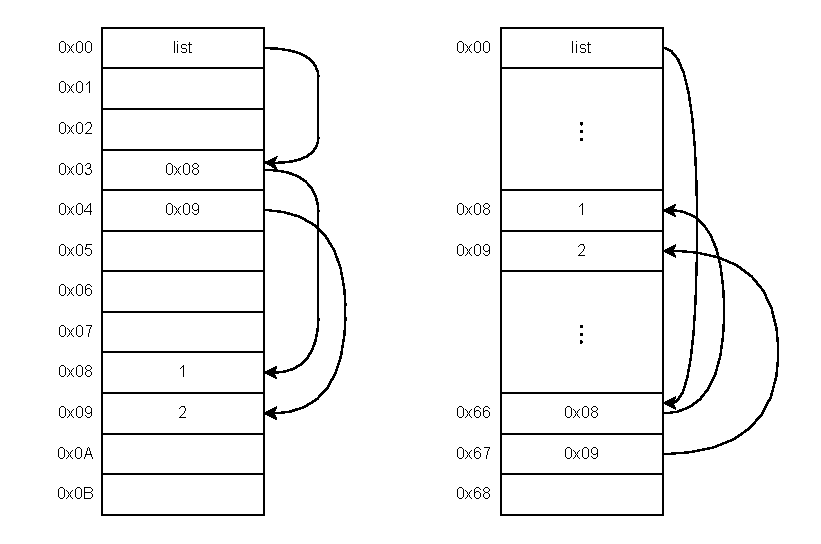
\includegraphics[width = \textwidth]{Figures/bor3.drawio.pdf}
    \caption{Memoria heap Java dopo il riallocamento dell'\texttt{ArrayList}.}
\end{figure}
%TODO Vedere lifetimes in Rust